\documentclass{article}
\usepackage{amsfonts}
\usepackage{amsthm}
\usepackage{amssymb}
\usepackage{amsmath}
\usepackage{graphicx}
\usepackage{subcaption}
\usepackage{xcolor}
\usepackage{mathtools}
\usepackage{ wasysym }
\usepackage{enumerate}
\usepackage{verbatim}


\numberwithin{equation}{section}
\newcommand{\new}[2]{
    \vspace{2mm}
    \noindent
    \textbf{
    \underline{#1}}
    \textit{{#2}}
    \
}

\def\<{{\langle}}
\def\>{{\rangle}}

\newcommand{\deriv}[2]{
\frac {d {#1} } {d {#2}}
}

\newcommand{\pderiv}[2]{
\frac {\partial {#1} } {\partial {#2}}
}

\DeclarePairedDelimiter\bra{\langle}{\rvert}
\DeclarePairedDelimiter\ket{\lvert}{\rangle}
\DeclarePairedDelimiterX\braket[2]{\langle}{\rangle}{#1\,\delimsize\vert\,\mathopen{}#2}


\newcommand{\textOr}{
    {
        \hspace{5mm}
        \textrm{or}
        \hspace{5mm}
    }
}

\newcommand{\textAnd}{
    {
        \hspace{5mm}
        \textrm{and}
        \hspace{5mm}
    }
}


\newcommand{\textWhere}{
    {
        \hspace{5mm}
        \textrm{where}
        \hspace{5mm}
    }
}



\newcommand{\Ixp}[1]{
    {
        e^{i{#1}}
    }
}



\newcommand{\halfFigure}[1]{
\begin{center}
\includegraphics[width = .5\linewidth]{{#1}}
\end{center}
}

\newcommand{\fullFigure}[1]{
\begin{center}
\includegraphics[width = .9\linewidth]{{#1}}
\end{center}
}

\def\twobytwoMat(#1, #2, #3, #4){
    {
        \begin{bmatrix}
            {#1} & {#2}\\
            {#3} & {#4}
        \end{bmatrix}
    }
}

\def\twobyoneMat(#1, #2){
    {
        \begin{bmatrix}
            {#1}\\
            {#2}
        \end{bmatrix}
    }
}

\def\twobytwoDet(#1, #2, #3, #4){
    {
        \begin{vmatrix}
            {#1} & {#2}\\
            {#3} & {#4}
        \end{vmatrix}
    }
}


\newcommand{\RR}{\mathbb{R}}
\newcommand{\CC}{\mathbb{C}}
\newcommand{\ZZ}{\mathbb{Z}}
\newcommand{\Zpos}{\mathbb{Z}_{pos}}
\newcommand{\NN}{\mathbb{N}}

\newtheorem{theorem}{Theorem}
\newtheorem{proposition}{Proposition}
\newtheorem{lemma}{Lemma}
\newtheorem{corollary}{Corollary}
\newtheorem{remark}{Remark}
\newtheorem{definition}{Definition}
\newtheorem{example}{Example}
\newtheorem{conjecture}{Conjecture}
\newtheorem{question}{Question}

\newcommand{\ch}{\text{ch}}

\begin{document}
\begin{center}
    \Large
    \textbf{301 Midterm}

    \large
    Daniel Son
\end{center}

\section{Section A}
\subsection*{A1) Math Fact}

\begin{proof}
    [Part a] 
    Split and switch order. It is easier done than said. 
    \begin{align}
        \int_{-a} ^a f(x) dx & = \ \int_0^a f(x) dx + \int_{-a}^0 
        f(x) dx \ \\ & = \  
        \int_0^a f(x) dx + \int_a^0 f(-x) (-dx) 
        \\ & = \
        \int_0^a \left(f(x) + f(-x)\right)dx 
        \ = \ 
        0
    \end{align}
    The integrand of the last integral vanishes since $f(x)$ is odd. 
\end{proof}

\begin{proof}
    [Part b] 
    Set $u = x - b$, then invoke the result from part a. 
    \begin{align}
        \int_{b - a}^{b + a} f(x - b) dx  \ = \ 
        \int_{-a}^{a} f(u) du \ = \ 0
    \end{align}
\end{proof}

\subsection*{A2) Photon Absorbtion} 
We first claim that we can ignore relativity for this problem. 
Upon inspection, the rest energy of the Rb atom is about 8 orders 
or magnitude greater than the kinetic energy added by the photon. 
Equate kinetic energy with the energy of a single photon. 

\begin{align}
    \frac 1 2 m v^2 \ = \ \frac {hc} {\lambda} \\ 
    v \ = \ \sqrt{\frac {2 c h}{m \lambda}}
\end{align}

Also, the following list of constants come in handy. 
\begin{align*}
    m & = \ 87 \ \rm amu \ = \ 87 \cdot 1.66 \cdot 10^{-27} kg \\
    c & = \ 3 \cdot 10^8 m/s \\ 
    h & = \ 6.626 \cdot 10^{-34} J/s \\ 
    \lambda & = \ 780 \ nm \ = \ 7.8 \cdot 10^{-7} m
\end{align*}

Thus, 
\begin{align}
    \boxed{
        v \ = \ 1879 m/s
    }
\end{align}

\subsection*{A3) Solar Radiation} 
As a preliminary, recall the Plank distribution. 
\begin{align}
    \rho(v, T) \ = \ \frac {8\pi v^2}{c^3}\frac{hv}{e^{hb/k_BT} - 1}
\end{align}

\begin{proof}
    [Part a]  \phantom{\qedhere}
\end{proof}
    \begin{figure}[h]
        \centering
        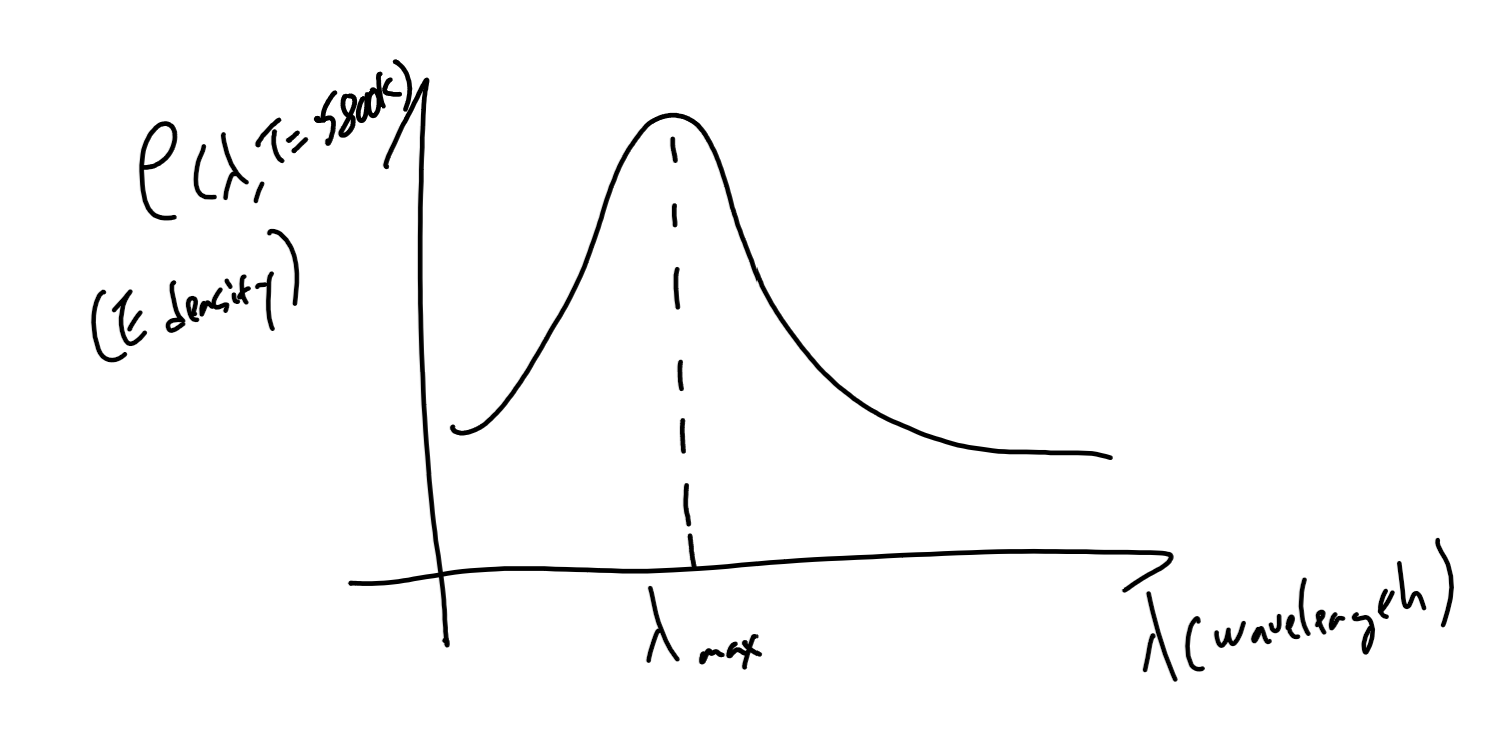
\includegraphics[width=0.8\textwidth]{A3_graph.png} % Replace 'figure.jpg' with your image file
        \caption{Sketch of the spectrum for part a}
        \label{fig:a3graph}
    \end{figure}
   
\begin{proof}
    [Part b] We wish to find the peak wavelength. From PS1, we have 
    computed the peak frequency. 
    \begin{align}
        \nu_{\rm pk} \ \approx \ \frac {2.82 k_B T} h
    \end{align}
    We derive the following expression for peak wavelength. 
    \begin{align} \boxed{
        \lambda_{\rm pk} \ = \ \frac {hc} {2.82 k_B T} \ = \ 880 \ nm }
    \end{align}
\end{proof}

\begin{proof}
    [Part c] If the wavelength ranges from $500 \ nm$ to $1100 \ nm$, then 
    the frequency ranges from $\nu_1 = c/1100 \ nm$ and $\nu_2 = c/500 \ nm$. 
    We set up an integral over the Plank distribution to find the fraction of energy 
    that will be absorbed. 
    \begin{align}\boxed{
        \int_{c/1100 \ nm}^{c / 500 \ nm } \rho(\nu, 5800K) d\nu}
    \end{align}
\end{proof}

\section{Section B}
\subsection*{B1) Single Photon Interference}
\begin{proof}
    [Part a] 
    A HeNe laser emits a light of wavelength $633\ nm$ with a power efficiency of 
    $P = 3\ mw$. The ray of light interacts with the intereferometer, 
    and reaches the APD where it is detected. The loss is 
    incurred by: 
    \begin{enumerate}
        \item Iris, loss of 50\% 
        \item ND filter, loss of $10^{-d}$ 
        \item APD detection efficiency, loss of 50\%
    \end{enumerate}

    We first count how much photons the laser emits. A single 
    photon has an energy of 
    \begin{align}
        E \ = \ pc \ = \ \frac {hc} \lambda
    \end{align}
    so the numerical frequency without losses are 
    \begin{align}
        P/E \ = \ \frac {P \lambda}{hc}.
    \end{align}
    Finally, we set up an equation, taking account of losses. 
    \begin{align}
        \frac {10^{-d}}{4} \frac {P \lambda}{hc} \ = \ 500 \ \rm Hz
    \end{align}
    Solve for $d$, the necessary index of the ND filter. 
    \begin{align}
        \boxed{
        d \ = \ -\log\left(
            \frac {hc}{P \lambda} \  2000 \ \rm Hz
        \right) \ \approx \ 12.68
        }
    \end{align}
\end{proof}

\begin{proof}[Part b-i]
    The linear gate accepts input from the 
    function generator and the APD. Whenever a photon is detected, 
    a pulse is sent to the linear gate, and the linear gate 
    sends the voltage of the function generator at the moment when 
    of detection. The function generator is also connected to the speaker, 
    and the voltage of the function generator corresponds to 
    the displacement of the moving leg. 

    The APD tallys the voltage information recieved from the linear 
    gate and outputs an histogram that displays the information 
    of photon counts for each bin of voltages\footnote{each 
    bin is a small interval of voltage}. 
\end{proof}


\begin{proof}
    [Part b-ii] 
    The plots of the background signal will not change 
    significantly. However, the interference signal would have 
    an additional cycle, i.e. the existing plot would be squished 
    to include about 2/3 of an additional sin function. This is 
    because the increase of the function generator voltage 
    increases the scan distance.  
    \begin{figure}[htp]
        \centering
        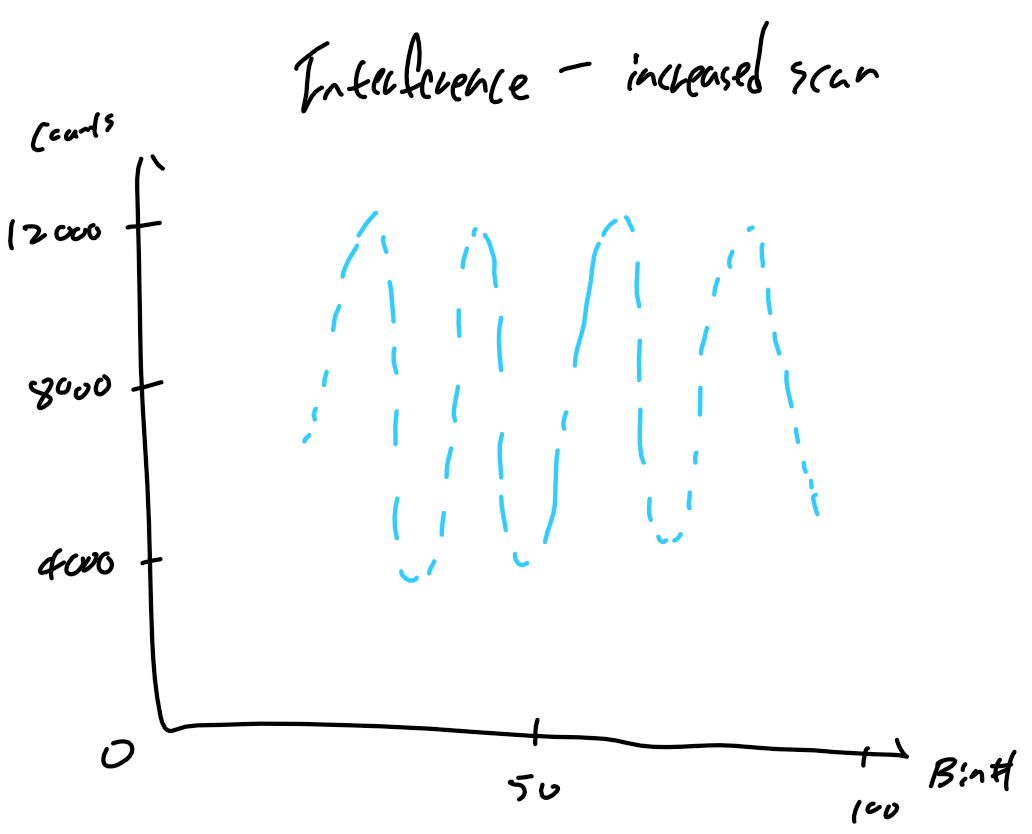
\includegraphics[width=0.8\textwidth]{B_spread.png} % Replace 'figure.jpg' with your image file
        \caption{Expected measurement for increased scan ($20\%$)}
        \label{fig:Bspread}
    \end{figure}
\end{proof}

\begin{proof}
    [Part b-iii] 
    \begin{figure}[htp]
        \centering
        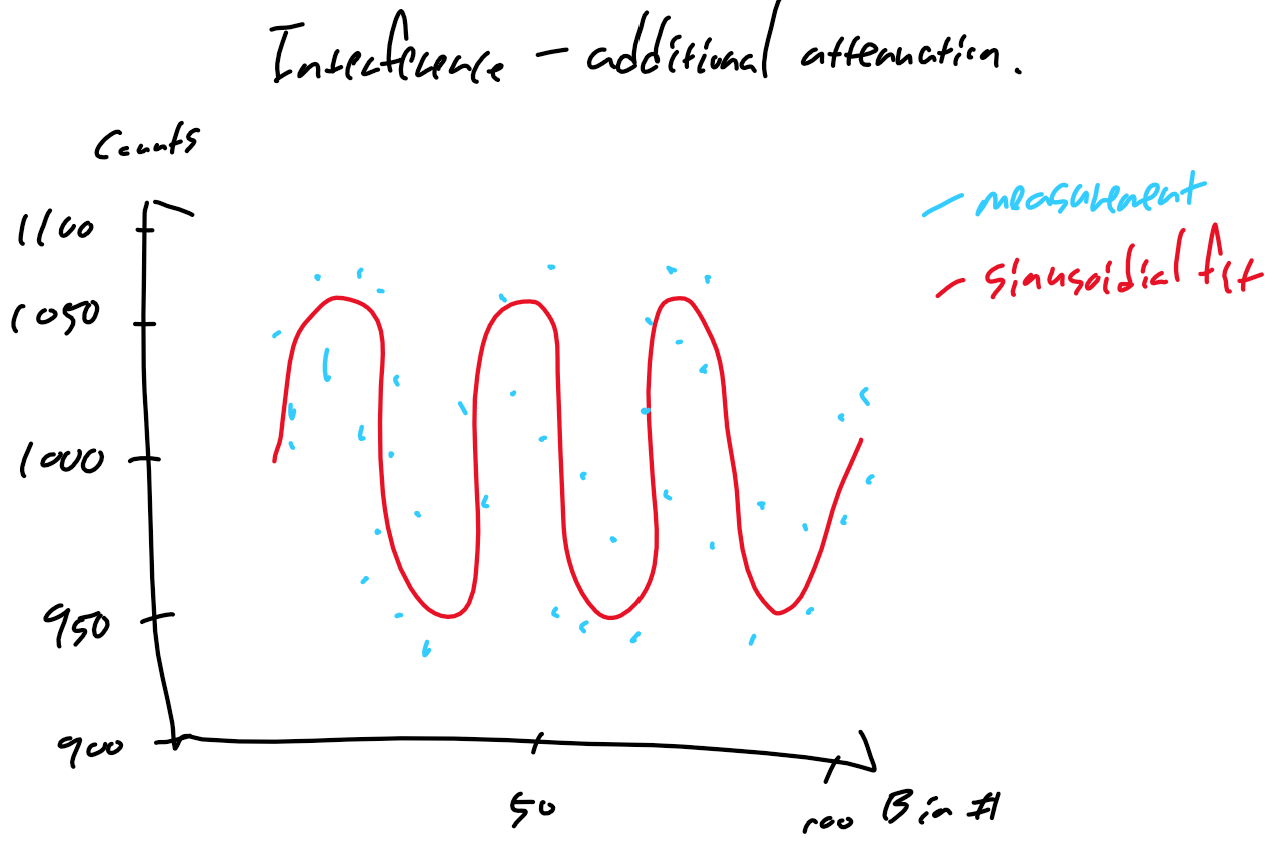
\includegraphics[width=0.8\textwidth]{B_ND.png} % Replace 'figure.jpg' with your image file
        \caption{Expected measurement for additional attenuation}
        \label{fig:Battenuated}
    \end{figure}

    
    \begin{figure}[htp]
        \centering
        \begin{subfigure}[b]{0.45\textwidth}
            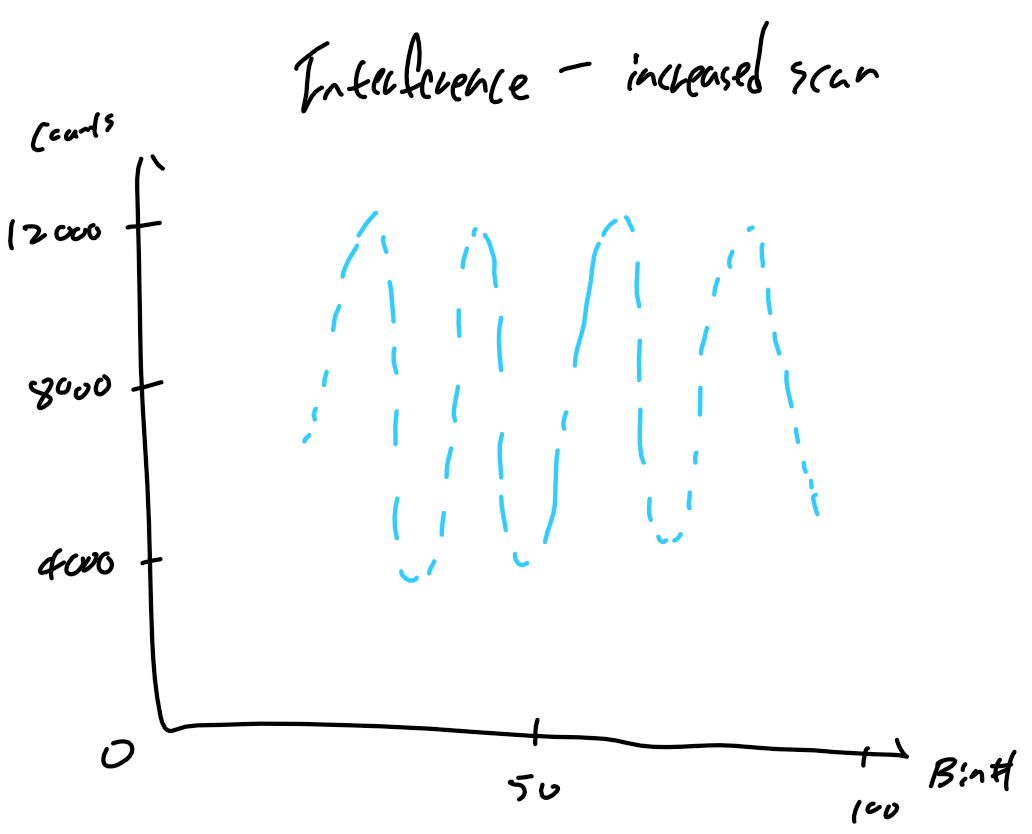
\includegraphics[width=\textwidth]{B_spread.png}
            \label{fig:fig1}
        \end{subfigure}
        \hfill
        \begin{subfigure}[b]{0.45\textwidth}
            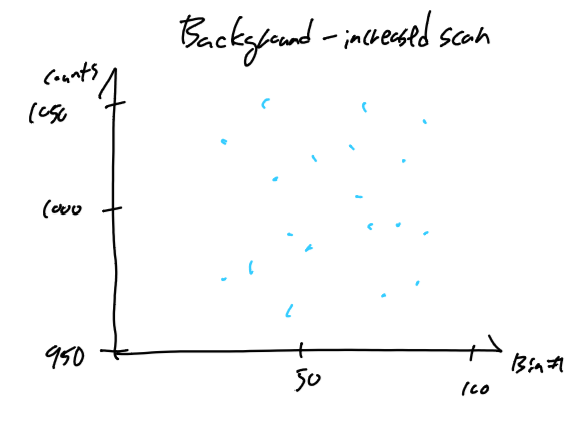
\includegraphics[width=\textwidth]{B_bg_spread.png}
            \label{fig:fig2}
        \end{subfigure}
        \
        \begin{subfigure}[b]{0.45\textwidth}
            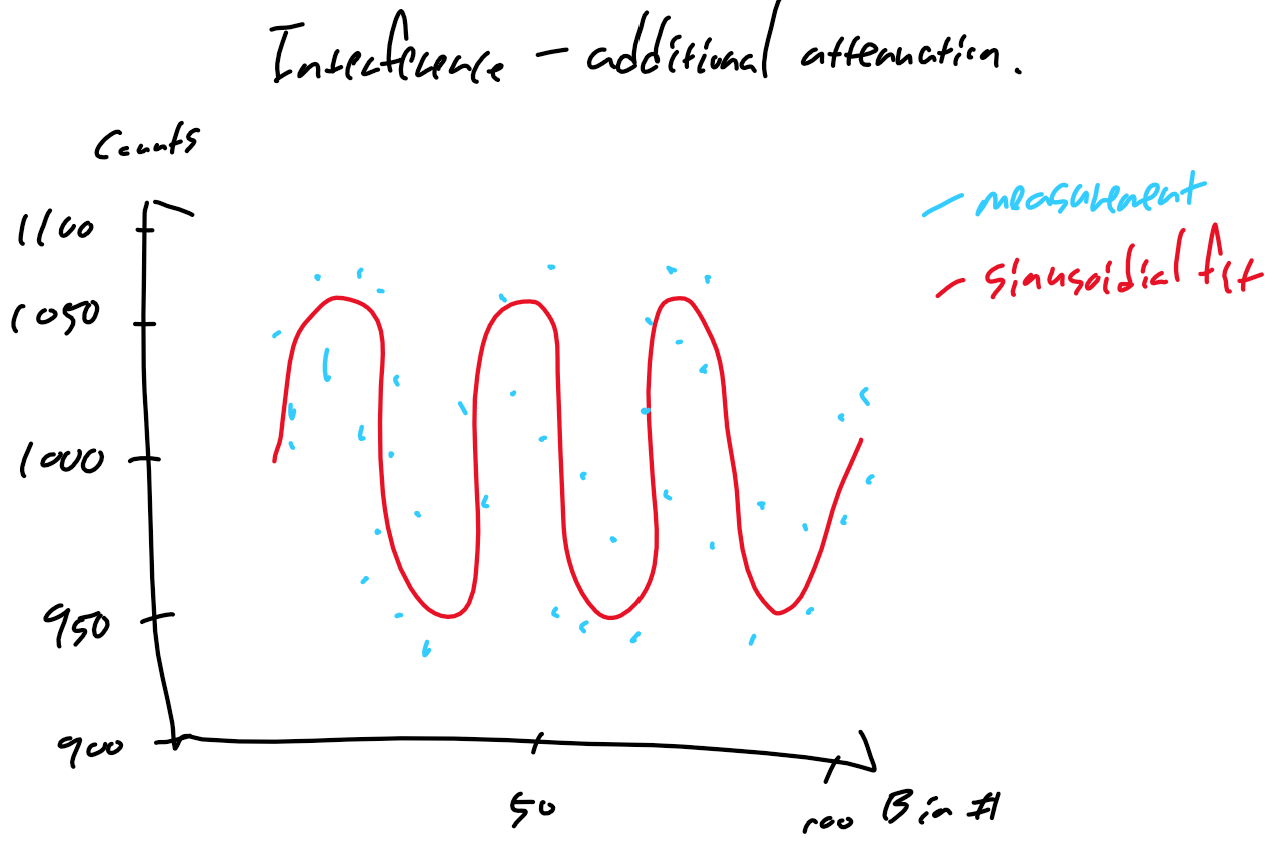
\includegraphics[width=\textwidth]{B_ND.png}
            \label{fig:fig3}
        \end{subfigure}
        \hfill
        \begin{subfigure}[b]{0.45\textwidth}
            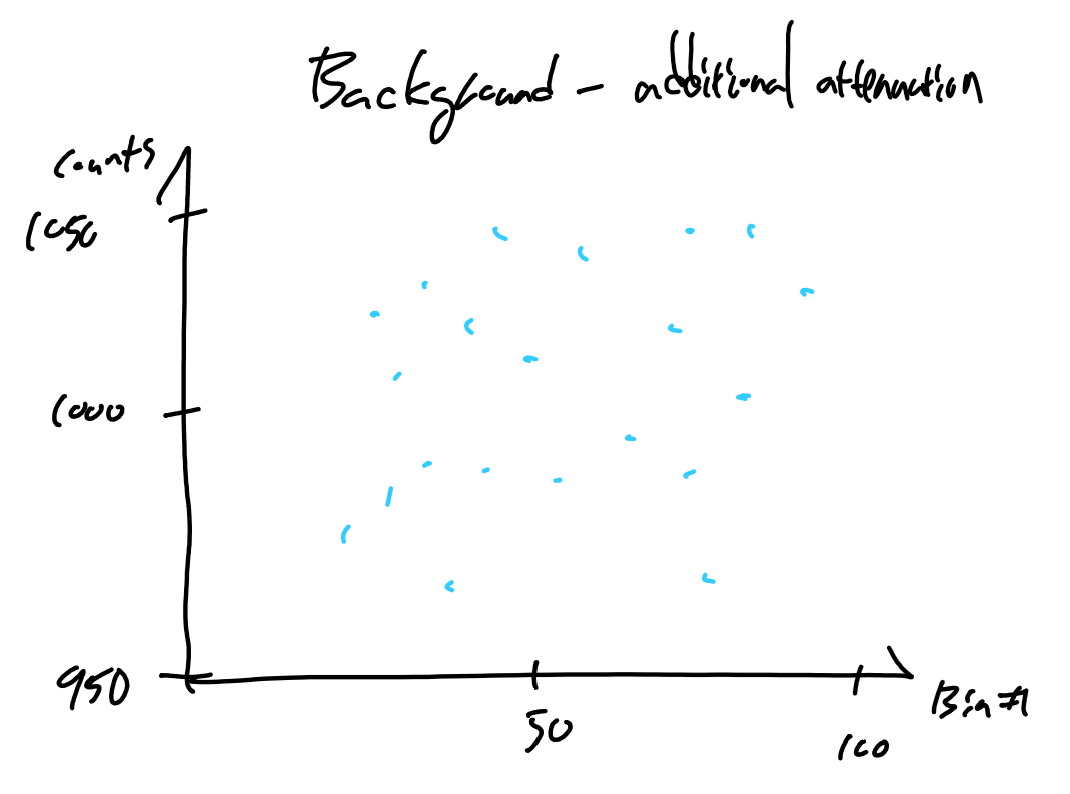
\includegraphics[width=\textwidth]{B_bg_ND.png}
            \label{fig:fig4}
        \end{subfigure}
    \end{figure}
    
    The peak to peak count of the interference signal before attenuation 
    is about $10000$ counts. An additional attenuation of ND2 will 
    decrease this count by a factor of $100$. Hence, the new 
    peak to peak difference of the count would be around 100. 
    Moreover, the background signal ranges around 1000 counts in average. 
\end{proof}

\begin{proof}
    Consider Feynman's description of the single slit experiment. 
    Single photons without interaction can be considered as 
    the distribution of bullets as a gunner randomly shoots toward 
    the screen. Without interference, the distribution would 
    be uniform, without an identifiable peak or valley, but only random noise. 
\end{proof}

\section{Section C}

\subsection*{C1) Free Particles and Fourier Transforms}

\begin{proof}
    [Part a]
\end{proof}
\begin{figure}[htp]
    \centering
    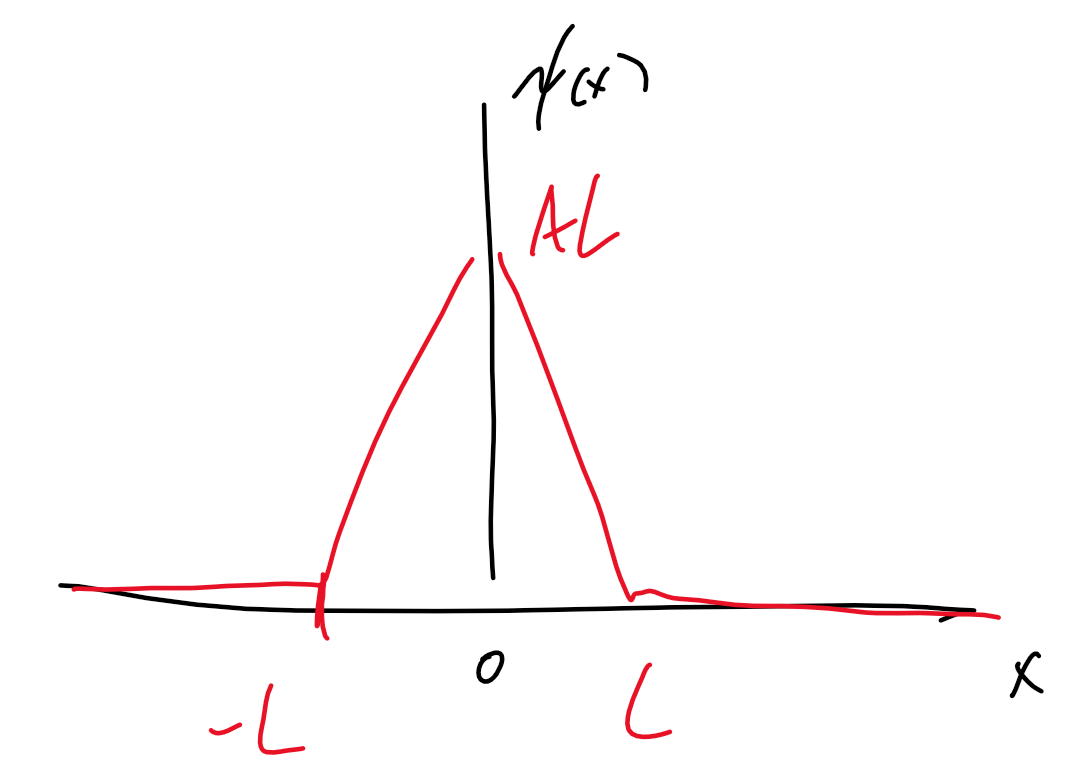
\includegraphics[width=0.8\textwidth]{C1_sketch.png} % Replace 'figure.jpg' with your image file
    \caption{Sketch of the wavefunction at $t = 0$}
\end{figure}

\begin{proof}
    [Part b]
    We compute the normalization constant by imposing the condition 
    that the integral of the square of the wavefunction must equal 1. 
    \begin{align}
        \int_{\mathbb R}\psi(x)^2 dx \ = \ 1 \\ 
        2 \int_0^L (L - x)^2 A^2 dx \ = \ 1 \\ 
        2A^2 \left[
            -\frac{(L - x)^3}{3}
        \right]_0^L \ = \ 1 \\ 
        \frac {2A^2 L^3} 3 \ = \ 1 \\ 
        \boxed{A = \sqrt{\frac 3 {2 L^3}}}
    \end{align}
\end{proof}

\begin{proof}
    [Part c]
    Clearly, $\psi(x)^2 x$ is odd. Thus, integrating 
    this function over the entirety of $\mathbb R$ should yield 
    zero. 
    \begin{align}
        \<x\> \ = \ 0
    \end{align} 

    The momentum can be computed via by-parts integration. 
    Recall the form of the momentum operator in position space. 
    \begin{align}
        p \ \equiv \ -i \hbar \nabla \textAnd p^2 \ \equiv \ -\hbar^2 \nabla^2
    \end{align}
    Our particle is 1D, so $\nabla = \pderiv{}{x}$. Consider the 
    following lines of algebra. 
    \begin{align}
        \<p^2\> \ = \ \int_{\mathbb R} \psi(x) (-\hbar^2 \nabla^2) \psi(x) dx \\ 
        = \ -\hbar^2 \int_{\RR} \psi(x) \psi''(x) dx  
    \end{align}
    Set $u = \psi(x)$, $dv = \psi''(x)dx$. 
    \begin{align}
        \<p^2\> \ = \ -\hbar^2 \left(uv - \int v du \right) \ = \ 
        -\hbar^2\psi(x)\psi'(x)\bigg|_{-\infty}^{\infty} + \hbar^2 \int_{\RR} \psi'(x)^2 dx \nonumber\\\label{eqn:fastInt}
        = \ \hbar^2 (A^2 2 L) \ = \ \boxed{\frac {3\hbar^2} {L^2}}
    \end{align}
    The last equality of \eqref{eqn:fastInt} follows 
    from the fact that $\psi'(x)$ is nonvanishing only at the 
    region $(-L, L)$.\footnote{To the timid mathematician who 
    worries that $\psi'(x)$ is undefined at $x = 0, \pm L$, we 
    assure that we can smoothen the function by infinesimal amount and take limits. }
\end{proof}

\begin{proof}
    [Part d]
    Take the Fourier transform of the wavefunction to obtain 
    an expression for $\phi(k)$. 
    \begin{align}
        \phi(k) \ = \ \mathcal F\{\psi(x)\}(k)
    \end{align}
    Unfold the definition and evaluate the integral. 
    \begin{align}
        \phi(k) & = \ \frac 1 {\sqrt{2 \pi }} 
        \int_{\RR} \psi(x) e^{-ikx} dx \\ 
        &= \ \frac 1 {\sqrt{2\pi}} 
        \left[
            \int_0^L A(L-x) e^{-ikx} dx 
            + 
            \int_{-L}^0 A(L - x) e^{-ikx}dx
        \right] \\ 
        &= \  \frac 1 {\sqrt{2\pi}} \int_0^L 2A(L - x) \cos(kx)dx 
    \end{align}
    Set up a by-parts integration table. 
    \begin{align*}
        {\rm sign} && u && dv \\ 
        \hline
        + && L - x && \cos(kx) \\ 
        - && -1 && \frac {\sin(kx)} k \\ 
        + && 0 && -\frac{\cos(kx)}{k^2}
    \end{align*}
    Finally, we have a closed form expression for $\psi(x)$. 
    \begin{align}
        \phi(k) & = \ \frac {2A}{\sqrt{2\pi}} \left[
            \frac {L - x} k \sin(kx) - \frac {\cos(kx)}{k^2}
        \right]_0^L \ = \ \frac {2A} {\sqrt{2 \pi }} \left[
            \frac 1 {k^2} - \frac{\cos(kL)} {k^2}
        \right] \\ 
            & = \boxed{
                \sqrt{
                    \frac {3L} {\pi}
                }\left(
                    \frac{1 - \cos(kL)}{(kL)^2}
                \right)
            }
    \end{align}
\end{proof}

\begin{proof}
    [Part e]
    The wavefunction starts as a $\wedge$ shape then disperses 
    to the entirety of $\RR$ in form of multiple sinuoidial bumps 
    with different amplitudes. This is because the wavefunction at 
    time $t = 0$ is composed of multiple energy eigenstates. Eigenstates 
    with higer energy disperse away from the center faster, and the others 
    move slower. 
\end{proof}


\subsection*{C2) Superpositions in the infinite well}

Remember that in an ISW, the $n$th energy eigenstate is the following. 
\begin{align}
    \psi_n(x) \ = \ \sqrt{\frac 2 a} \sin\left(\frac {n \pi x} a\right)
\end{align}

\begin{proof}
    [Part a]
    Invoke orthonormality of the energy eigenstates. 
    \begin{align}
        \int_\RR \psi_A(x)^2 dx = 1 \\ 
        N^2 \left[
            \int 3 \psi_1^2(x) dx + \int \psi_3^2(x) dx - \sqrt 3 
            \int \psi_1(x)\psi_3(x) dx 
        \right] = 1 \\ 
        4N^2 \ = \ 1 \\ 
        \boxed{
        N\ = \ \frac 1 2}
    \end{align}
\end{proof}

\begin{proof}
    [Part b]\textcolor{blue}{
    There are no hopes that either of $\psi_A$ or $\psi_B$ 
    are eigenstates of $\hat p\equiv i\hbar \nabla$.} The spacial 
    derivative converts the sin terms to cosine, and a constant 
    multiple of the sin function cannot generate a cosine function. 
    
    \textcolor{blue}{$\psi_B$ is an eigenstate of $\hat p^2$, while $\psi_A$ is not. }
    $\psi_B$ is an energy eigenstate, and within the well, 
    the potential is zero so $E = p^2/2m$ and the energy operator 
    is a constant multiple of $\hat p^2$. $\psi_A$ is not an 
    energy eigenstate, so it cannot be an eigenstate of $\hat p^2$. 
\end{proof}

\begin{proof}
    [Part c] 
    For a mixed state, the time dependent wavefunction can 
    be retrieved by decomposing the time independent solutions 
    into energy eigenstates and invoking time evolution for 
    each energies. We already have an eigendecomposition. 

    The time evolution function is 
    \begin{align}
        T_n(t) \ = \ \exp\left(-\frac{iE_n t} \hbar\right) \\ 
        E_n \ = \ \frac{n^2 \hbar^2 \pi^2}{2 m a^2}
    \end{align}
    for the $n$th energy eigenstate. 

    We write out the time dependent wavefunctions. 
    \begin{align}
        \Psi_A(x, t) \ = \ 
        \sqrt{\frac 1 {2a}} \left[-\sqrt{3}\sin\left(\frac{\pi x} a \right) 
        \exp\left(-\frac{ i \hbar \pi^2 t}{2 m a^2}\right) 
        + \sin\left(\frac{3 \pi x} a \right) 
        \exp\left(-\frac{ 9 i \hbar \pi^2 t}{2 m a^2}\right) 
        \right] \\ 
        \Psi_B(x, t) \ = \ 
        \sqrt{\frac 2 a} \sin\left(\frac{2\pi x} a \right) 
        \exp\left(-\frac{2 i \hbar \pi^2 t}{m a^2}\right) 
    \end{align}
\end{proof}

\begin{proof}
    [Part d]
    The particle collapses into one of the energy eigenstates, 
    either $\psi_1$ or $\psi_3$. The possible energy measurements are 
    \begin{align}
        E_1 \ = \ \frac{\hbar^2 \pi^2}{2 m a^2} \textAnd 
        E_3 \ = \ \frac{9 \hbar^2 \pi^2}{2 m a^2}
    \end{align}

    We compute the probability of this 
    probability by the Born probability rule. 

    \begin{align}
        P(A\rightarrow 1) \ = \ \<\psi_A|\psi_1\>^2 \ = \ \left(\frac {\sqrt 3} 2\right)^2 \ = \ \frac 3 4
        \\
        P(A \rightarrow 3) \ = \ \<\psi_A|\psi_3\>^2 \ = \ \left(\frac 1 2\right)^2 \ = \ \frac 1 4
    \end{align}

    The state of the particle after measurement is the 
    first or the third energy eigenstate, which is either 
    \begin{align}
        \psi_1(x) T_1(t) \textOr \psi_3(x) T_3(t).
    \end{align}
\end{proof}

\begin{proof}
    [Part e] 
    Classical probability comes to the rescue. 
    \begin{align}
        \Delta E \ = \ \sqrt{\<E^2\> - \<E\>^2}
    \end{align}
    We know that $E_3 = 3E_1$ and that the probability of 
    the wavefunction collapsing into the third energy eigenstate 
    is $1/4$. 
    \begin{align}
        \<E\> \ = \ \frac {3} 4 E_1 + \frac{1} 4 E_3 \ = \ \frac {3 + 9} 4 E_1 \ = \ 3E_1 \\ 
        \<E^2\> \ = \ \frac {3} 4 E_1^2 + \frac 1 4 E_3^2 \ = \ \frac {3 + 81} 4 E_1^2 \ = \ 21 E_1^2 \\ 
        \boxed{\Delta E \ = \ \sqrt{21 - 9} E_1 \ = \ 2\sqrt 3 E_1 \ = \ \frac{\sqrt{3} \hbar^2 \pi^2}{m a^2}}
    \end{align}
\end{proof}

\begin{proof}
    [Part f] 
    The probability densities of $\Psi_A$ are time dependent, 
    while the probability density of $\Psi_B$ is time independent. 
    This is because $\psi_B$ is in a pure state and the wavefunction 
    can be brought to the same shape under some phase shift. However, for 
    $\Psi_B$, the two energy eigenstate evolve in a different speed, 
    and the interaction between the two deforms the wavefunction 
    such that a constant phase shift cannot bring the wavefunction to 
    the initial form. 

    The frequency of the oscillation of the amplitude $|\Psi_A|^2$ is 
    determined by the frequency of the lowest eigenstate.\footnote{This 
    does not hold in full generality, but only because $1$ is 
    an integer multiple of $1/3^2$ in this case.} Let $\tau$ 
    denote the period, and $f$ the frequency. 
    \begin{align}
        \frac {E_1 \tau} \hbar \ = \ 2 \pi \\ 
        \boxed{f \ = \ \frac 1 \tau \ = \ \frac {E_1}{2 \pi \hbar} \ = \ \frac{\hbar \pi }{4 m a^2}}
    \end{align}
\end{proof}

\begin{proof}
    [Part g]
    \textcolor{blue}{Both the position and momentum are time independent}. 
    Relabel the axis such that the new zero is the center of the well. 
    Then, both the first and the third energy eigenstates have an 
    even symmetry. The same goes for their derivates. The superposition 
    of the first and the third eigenstate, regarless of the phase 
    difference imposed by time evolution, must also be even. Hence 
    the expected value of both of these observables are zero in the 
    relabeled space. 
\end{proof}

\subsection*{C3) Uncertainty and Bound States}
\begin{proof}
    [Part a]
    Write out the time independent Schrodinger equation to provide a 
    condition for the energy eigenstates. 
    \begin{align}
        E\psi(x) \ = \ -\frac{\hbar^2}{2m} \psi''(x) + V(x) \psi(x)
    \end{align}
    Solve for $V(x)$ and impose even symmetry. 
    \begin{align}
        V(x) & = \ E + \frac{\hbar^2}{2m} \frac{\psi''(x)}{\psi(x)} 
        \\ V(x) & = \ V(-x) \textOr 
        E + \frac{\hbar^2}{2m} \frac{\psi''(x)}{\psi(x)}  \ = \ 
\frac{\hbar^2}{2m} \frac{\psi''(-x)}{\psi(-x)} 
    \end{align}
    We obtain a nice condition for $\psi(x)$. 
\begin{align}\label{eqn:c3symm}
        \psi''(x) \psi(-x) \ = \ \psi''(-x)\psi(x)
\end{align}
Since $\psi(x)$ is a bounded particle, 
it is possible to expand the function into 
sum of sines and cosines. For simplicity, 
suppose the particle is bounded in the region $[-\pi, \pi]$. 

\begin{align}
    \psi(x) & = \ \sum_n a_n \sin(nx) + \sum_n b_n \cos(nx) + C \\ 
    \psi''(x) & = \ -\sum_n a_n n^2 \sin(nx) - \sum_n b_n n^2 \cos(nx) 
\end{align}

Suppose the constant offset $C$ is nonzero, and 
compare the coefficient of $\sin(nx)$ from \eqref{eqn:c3symm}. 
\begin{align}
    -Ca_n n^2 \ = \ C a_n n^2 
\end{align}
Hence the $a_n$ terms vanish and $\psi(x)$ is a sum of cosines, 
thus even. Now, suppose there exists some $a_n \neq 0$. Then, 
we compare the coefficient of $\sin(nx)\cos(mx)$ for any $m$. 
\begin{align}
    -a_n b_m n^2 m^2 \ = \  a_n b_m n^2 m^2
\end{align}
So $b_m$ vanishes and $\psi(x)$ is a sum of sines, hence odd. 

This means that the probability amplitude $\psi(x)^2$ is always 
even. The expected value of $x$ over any even probability distribution 
defined over $\RR$ must be zero. Thus, 
\begin{align}
    \<x\> \ = \ 0
\end{align}

\textcolor{blue}{Extra Credit:} Suppose $\Psi(x, t)$ 
is a general state that is not necessarily pure. Then, 
the time average expectation value can be computed as follows. 

\begin{align}
    \<x\> & = \ \int_T \int_\RR \Psi(x, t)^*x \Psi(x, t)dx \ dt \\ 
    & \int_T \int_\RR \left(\sum_n \psi_n(x) e^{iE_n/\hbar t} \right) x \left(\sum_m \psi_m(x)e^{-iE_m/\hbar t}\right) dx \ dt
\end{align}

The cross terms involving $\psi_n(x)\psi_m(x)$ dies out 
when taking long time averages, since the oscillations do not cancel out, 
i.e. $e^{-i(E_n - E_m)/\hbar t}$ is not constant. 
\begin{align}
    \<x\> \ =\ \sum_n \int_\RR x \psi_n(x)^2 dx \ =\  0
\end{align}
Each of the component integrals are zero, for they are the 
expected position of each energy eigenstate. 
\end{proof}

\begin{proof}
    [Part b]
    \begin{align}
        \Delta x \ = \ \sqrt{\<x^2\> - \<x\>^2} \ = \ \sqrt{\<x^2\>} \ = \ x_{\rm RMS}
    \end{align}
    The crux of the argument is that $\<x\> = 0$. 
\end{proof}

\begin{proof}
    [Part c]
    Considering the Fourier expansion of a function, we notice 
    that a derivative of an even function must be odd and 
    the derivative of an odd function must be even. With this 
    in mind, compute $\<p\>$ for an eigenstate. 
    \begin{align}
        \<p\> \ = \ \int_\RR \psi(x) (-i\hbar)\deriv {}{x} \psi(x) dx 
        \ = \ -i\hbar \int_\RR\psi(x)\psi'(x) dx \ = \ 0 
    \end{align}
    The last equality follows because integrating an odd function 
    over $\RR$ yields zero. For nonpure states, we can repeat the 
    argument in part a to obtain the same result.
\begin{align}
        \Delta p \ = \ \sqrt{\<p^2\> - \<p\>^2} \ = \ \sqrt{\<p^2\>} \ = \ x_{\rm typical}
    \end{align}
 \textcolor{blue}
    {Note that for nonpure states, this result holds only for time average values of uncertainty. }
    \begin{align}
        \Delta p \ \sim \ p_{\rm typical}
    \end{align}
\end{proof}

\begin{proof}
    [Part d-i]
    The quantity $\Delta x \Delta p = x_{\rm RMS} p_{\rm typical}$ 
    resembles the angular momentum of the particle. The lowest 
    energy eigenstate has the lowest energy, and it is reasonable to say 
    that a particle in this state must have the lowest angular momentum. 
\end{proof}
\begin{proof}
    [Part d-ii] Bash out the expected value computation. 
    \begin{align}
        E & = \ \<p^2\>/2m + \<V(x)\> \\
        & = \ p_{\rm typical}^2/2m + \frac {m \omega^2} 2\<x^2\> \\ 
        & = 
            p_{\rm typical}^2/2m + \frac {m \omega^2} 2x_{\rm RMS}^2 \\\label{eqn:C3Eexact}
        & = 
        \frac \hbar {2m x_{\rm RMS}^2} + \frac {m \omega^2 x_{\rm RMS}^2} 2 
    \end{align}
    We wish to find the minimum value of this energy. Consider the 
    following function $f:\RR_{\rm pos} \rightarrow \RR$. 
    \begin{align}
        f(u) \ = \ u + \frac 1 u 
    \end{align}
    This function achieves minimum of 2 at $u = 1$.\footnote{
        This is a calculus proof. $f'(1) = 0$ and indeed $u = 1$ 
        is a global minimum upon inspection. 
    }
    For some constants $\alpha, \beta$, we can rewrite the energy as 
    follows. 
    \begin{align}
        E(x_{\rm RMS}^2) \ = \ \alpha\left(
            \frac 1 {\beta x_{\rm RMS}^2 } + \beta x_{\rm RMS}^2 \right)\ = 
            \ \alpha f(\beta x_{\rm RMS}^2)
    \end{align}
    By comparison with \eqref{eqn:C3Eexact}, we write 
    \begin{align}
        \alpha \beta \ = \ \frac {m \omega^2} 2 \textAnd \beta / \alpha \ = \ \frac{2m} {\hbar^2} \\ 
        \alpha \ = \ \sqrt{\frac {m \omega^2 \hbar^2}{4m}} \ = \ \frac {\hbar\omega} 2
    \end{align}
    The minimum energy is $2\alpha$. 
    \begin{align}
        \boxed{
            E \ = \ \hbar \omega
        }
    \end{align}
    
\end{proof}


\subsection*{C4) Half Infinite Well}

\begin{proof}
    [Part a, b]
    \begin{figure}[htp]
        \centering
        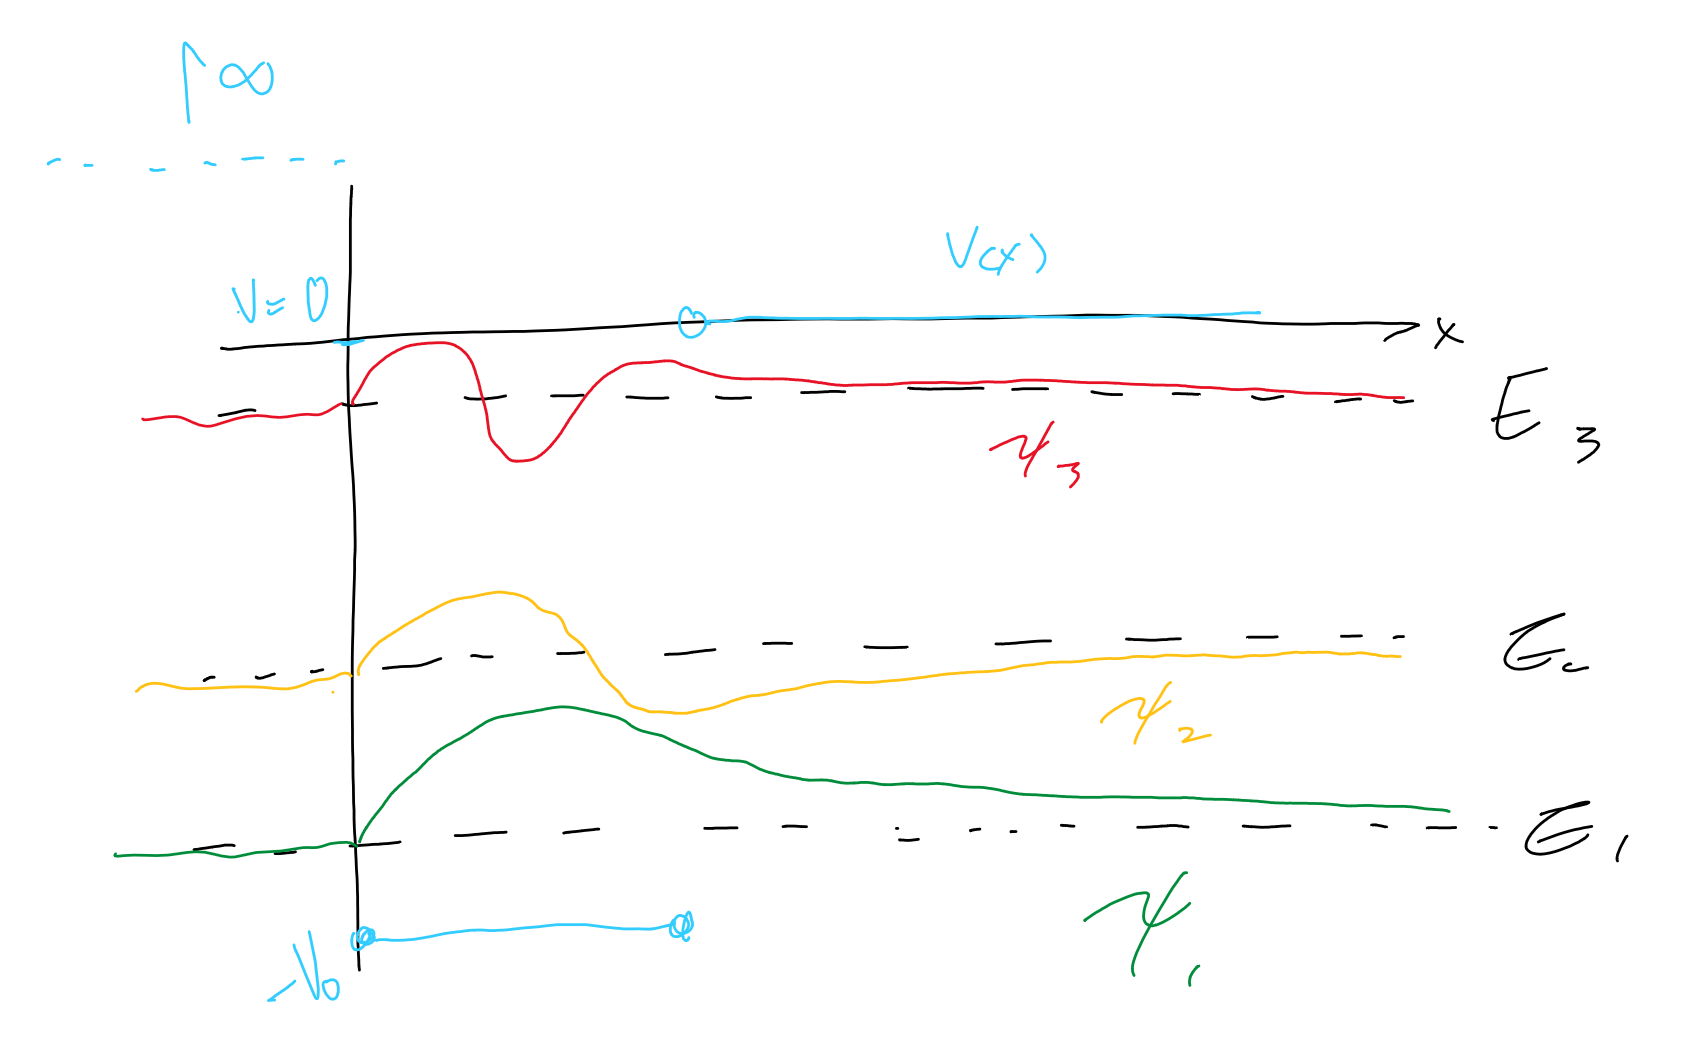
\includegraphics[width=0.8\textwidth]{C4_Potential.png} % Replace 'figure.jpg' with your image file
        \caption{The Half infinite potential and the first three energy eigenstates. }
        \label{fig:example}
    \end{figure}
    
    Both of the three eigenstates vanish at region I where 
    the potential is infinite. On region II, it displays 
    oscillatory behavior, where the first mode has 
    one node, second mode has two, and the third has three. 
    On region III, the potentials die out exponentially. 
\end{proof}

\begin{proof}
    [Part c] 
    \begin{align}\label{eqn:c4SE}
        E\psi & = \ -\frac {\hbar^2}{2m} \psi'' + \infty\psi && \text{Region I} \\ 
        E\psi & = \ -\frac {\hbar^2}{2m} \psi'' - V_0\psi && \text{Region II} \\ 
        E\psi & = \ -\frac {\hbar^2}{2m} \psi''  && \text{Region III} 
    \end{align}

\end{proof}

    The wavefunction vanishes at Region I.\footnote{
        It feels queasy to write $\infty$ as a number, 
        but it shows the fact that $\psi$ cannot be nonvanishing at the region.
    }

    Since $E < 0$, we notice that the equation for Region II is 
    exactly a SHO, and has a complex exponential solution. Region III 
    is similar, but the solution is a regular exponential. Exponential 
    growth at $x \rightarrow \infty$ is not plausible, so the solution 
    must be a negative exponential. Thus, the time independent 
    solution must be in the following form. 
    \begin{align}
        \psi(x) \ = \ \begin{cases}
            0 & (x < 0) \\ 
            A \sin(kx) & (0 \leq x \leq L) \\ 
            B e^{-qx} & (x \geq L)
        \end{cases}
    \end{align}
    
\begin{proof}
    [Part d]
    The wavefunction is continuous and differentiable at point $x = L$. 
    \begin{align}\boxed{
        \psi(L_-) \ = \ \psi(L_+) 
        \textAnd 
        \psi'(L_-) \ = \ \psi'(L_+)
    }
    \end{align}
\end{proof}

We do some more work before we provide a solution for the last part. 
The boundary condition can be solved as follows. 
\begin{align}\label{eqn:c4bdry}
    A \sin(kL) & = \ B e^{-qL} \\ 
    A \cos(kL) & = \ -\frac q k B e^{-qL}
\end{align}

Also, the energy can be written in terms of $k, q$ by \eqref{eqn:c4SE}. 
\begin{align}
    E & = \ -\frac{\hbar^2 q^2} {2m} \\\label{eqn:c4energies}
    E & = \ \frac{\hbar^2 k^2}{2m} - V_0
\end{align}

Introduce the following subsititution. 
\begin{align}
    R & = \ L \sqrt{k^2 + q^2} \\ 
    y & = \ kL
\end{align}

Note that $R$ depends on $V_0$. 
\begin{align}
    R \ = \ \frac L \hbar \sqrt{2m V_0}
\end{align}

\begin{proof}
    [Part e-i]
    We suspect that if $L\rightarrow 0$ or $V_0 \rightarrow \infty$, 
    then the wavefunction must approach an infinite square well.\footnote{
        The first condition $L \rightarrow 0$ is disputable, since 
        if the well width goes to zero, then the well disappears. 
    }
\end{proof}

\begin{proof}
    [Part e-ii] We wish to show that the energies of the 
    wavefunction approach those of an infinite square well as $V_0 \rightarrow \infty$. 
    From \eqref{eqn:c4energies}, we notice that the energies 
    already resemble the ISW case but with a constant offset of $V_0$. 
    For the previous solution of the ISW, we assumed that the bottom 
    of the well has a potential of zero. For the limiting case 
    of the half infinite well, the bottom potential is $V_0$, so 
    we can ignore this constant offset. It suffices to show that 
    $k = n\pi/L$ for eigenstates. 

    From the boundary conditions stated in \eqref{eqn:c4bdry}, 
    we can deduce 
    \begin{align}
        A\sin(kL) + \frac {Ak} q \cos(kL) \ = \ 0 \\ 
        \frac y {\sqrt{R^2 - y^2}} \ = \ -\tan(kL) \\\label{eqn:c4circle}
        -y \cot(y) \ = \ \sqrt{R^2 - y^2}
    \end{align}

    As $V_0\rightarrow \infty$, $R \rightarrow \infty$, and 
    the RHS of \eqref{eqn:c4circle} becomes an infinitely 
    large semicircle, which can be considered as a horizontal 
    line at infinity. $-y\cot(y)$ approaches infinity at $y = n\pi, (n = 1, 2, 3, \dots)$. 
    Therefore, \begin{align}
        \boxed{k \ = \ \frac{n\pi} L}
    \end{align}
    and this yields
    \begin{align}
        E_n \ = \ \frac{n^2 \hbar^2 \pi^2}{2m L^2} - V_0
    \end{align}
    which is exactly the energy levels of the $n$th eigenstate 
    of a ISW where the bottom potential is $V_0$ and the well width is $L$. 

    In the limiting case of the Half Infinite Well with width $L$, 
    \begin{align}
        \boxed{L \ = \ l}
    \end{align}
    where $l$ is the width of an ISW. That is, the width of 
    the two wells match. 
\end{proof}


\end{document}